\section{Descripción no formal}\label{sec:dnf}
Para simplificar la explicación del algoritmo veremos $x$ e $y$ como vectores de caracteres. El primer carácter de $x$ será $x[0]$ y el último $x[m-1]$.\\

El algoritmo comparará los caracteres del patrón de derecha a izquierda empezando por el que está más a la derecha. De esta manera el algoritmo empezará comparando el carácter $x[m-1]$ con el carácter $y[m-1]$. Si se encuentran dos carácteres diferentes, o ambas cadenas coinciden, se usarán dos funciones para mover el patrón a la derecha respecto al texto. Estas funciones son conocidas por los nombres \textbf{good-suffix shift} (movimiento del buen sufijo) y \textbf{bad-character shift} (movimiento del mal caracter).\\ 

Supongamos que $x[0]$ está alineado con $y[j]$, y encontramos el primer carácter diferente (buscando desde la derecha) en la posición $x[i] = a \neq y[j+i] = b$. Por lo tanto, $x[i+1 \ \  ... \ \  m-1] = y[j+i+1 \ \  ... \ \  j+m-1] = u$. El \textit{good-suffix shift} consiste en alinear el segmento $y[j+i+1  ...  j+m-1]$ con otra aparición suya en $x$ que cumpla que el carácter que le precede es diferente a $x[i] = a$. Si hay varias, cogemos la que se encuentre más a la derecha (ver figura \ref{gss1}).\\ 

\begin{figure}[H]
  \centering
    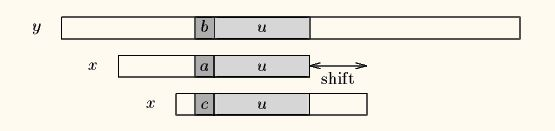
\includegraphics[width=0.7\textwidth]{gss1}
  \caption{Good-suffix shift, $u$ vuelve a aparecer en $x$ precedido por un carácter $c \neq a$}
	\label{gss1}
\end{figure}

Si no existe ese tipo de segmento, el movimiento consistirá en alinear el mayor sufijo $v$ de $y[j+i+1 \ \  ... \ \  j+m-1]$ con un prefijo coincidente de $x$ (ver figura \ref{gss2}).\\

\begin{figure}[H]
  \centering
    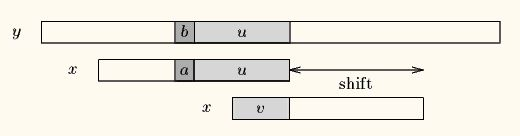
\includegraphics[width=0.7\textwidth]{gss2}
  \caption{Good-suffix shift, un sufijo de $u$ reaparece al principo de $x$}
	\label{gss2}
\end{figure}

El \textit{bad-character shift} consiste en alinear el carácter $y[i+j]$ con su aparición más a la derecha en $x[1 \ \  ... \ \  m-2]$ (ver figura \ref{bcs1}).\\

\begin{figure}[H]
  \centering
    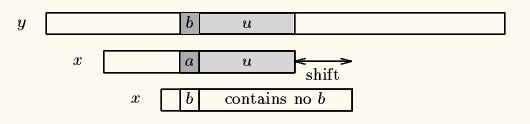
\includegraphics[width=0.7\textwidth]{bcs1}
  \caption{Bad-character shift, $b$ aparece en $x$}
	\label{bcs1}
\end{figure}

Si $y[i+j]$ no aparece en $x$, no habrá alineación posible de $x$ con $y[i+j]$, por lo que alinearemos $x[0]$ con $y[i+j+1]$(ver figura \ref{bcs2}).\\

\begin{figure}[H]
  \centering
    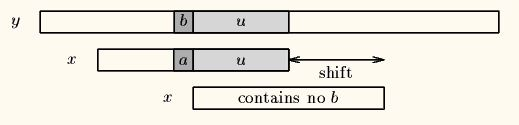
\includegraphics[width=0.7\textwidth]{bcs2}
  \caption{Bad-character shift, $b$ no aparece en $x$}
	\label{bcs2}
\end{figure}

Es interesante darse cuenta de que el \textit{bad-character shift} puede ser negativo, por lo tanto, el algoritmo elegirá el máximo valor arrojado por el \textit{good-suffix shift} y el \textit{bad-character shift} a la hora de hacer avanzar $x$ respecto a $y$.


%%%%%%%%%%Ejemplo%%%%%%%%%%
\subsection{Ejemplo del algoritmo de Boyer-Moore}
A continuación, se mostrará gráficamente el funcionamiento del algoritmo para un ejemplo concreto buscando un patrón en un texto en inglés. En cada paso, marcaremos con negrita el carácter en el que el algoritmo centra su atención.\\

\begin{align*} 
&x:     & &AT-THA\textbf{T}\\
&y: ... & &WHICH-\textbf{F}INALLY-HALTS.--AT-THAT-POINT ...\\
\end{align*}

Como `F' no aparece en $x$, usamos un \textit{bad-character-shift} (ver figura \ref{bcs2}) y desplazamos $x$:\\

\begin{align*} 
&x:     &        &AT-THA\ \textbf{T}\\
&y: ... & WHICH-F&INA\ LL\ Y\ \textbf{-}HALTS.--AT-THAT-POINT \ ...\\
\end{align*}

Ahora usamos otro \textit{bad-character-shift} (ver figura \ref{bcs1}) y desplazamos $x$ para alinear el espacio (-) de $y$ con el primer espacio (desde la derecha) de $x$:\\

\begin{align*} 
&x:     &        		 AT&-THA\textbf{T}\\
&y: ... & WHICH-FINALLY&-HAL\textbf{T}S.--AT-THAT-POINT ...\\
\end{align*}

Observamos que los caracteres visitados coinciden, por lo que movemos nuestra atención un carácter hacia la izquierda:\\

\begin{align*} 
&x:     &        		 AT&-TH\textbf{A}T\\
&y: ... & WHICH-FINALLY&-HA\textbf{L}TS.--AT-THAT-POINT ...\\
\end{align*}

Hacemos un \textit{bad-character-shift} (ver figura \ref{bcs2}) y, como `L' no aparece en $x$, avanzamos $m$ posiciones:\\

\begin{align*} 
&x:     &        					 &AT-THA\textbf{T}\\
&y: ... & WHICH-FINALLY-HAL&TS.\ \ --A\textbf{T}-THAT-POINT ...\\
\end{align*}

Ahora vemos que son los dos últimos caracteres de $x$ los que coinciden con $y$, por lo que movemos nuestra atención $2$ caracteres a la izquierda:\\

\begin{align*} 
&x:     &        					 &AT-T\textbf{H}AT\\
&y: ... & WHICH-FINALLY-HAL&TS.\ \ -\textbf{-}AT-THAT-POINT ...\\
\end{align*}

Finalmente, usamos un \textit{good-suffix-shift} (ver figura \ref{gss2}) de forma que encontramos una aparición de $x$ en $y$:\\

\begin{align*} 
&x:     &        				     	  &AT-THA\textbf{T}\\
&y: ... & WHICH-FINALLY-HALTS.--&AT-THA\textbf{T}-POINT ...\\
\end{align*}

Hemos de notar que solo hemos referenciado $y$ 14 veces, de las cuales 7 han sido para realizar la última comparación. Las otras 7 nos han permitido pasar los primeros 22 caracteres de $y$.

